\chapter{이징 상관관계, 평균장, 자발 자화}

\lectureoverview{1차원 이징 사슬은 각 격자점의 스핀을 결합 변수로 바꾸면 정확히 풀 수 있다. 이 변수 변환으로 분배 함수는 곱으로 바뀌며, 유한한 모든 온도에서 상관관계가 지수적으로 감소함을 알 수 있다. 고차원 격자에서는 각 스핀이 많은 이웃으로부터 영향을 받으므로 거동이 달라진다. 이웃들의 영향을 평균장으로 다루면 자기일관 방정식과 평균장 임계온도를 얻을 수 있고, 임의로 작은 외부장이 자화된 상 가운데 하나를 어떻게 선택하는지도 정밀하게 설명할 수 있다.}

\section{이징이 실제로 발견한 것}

역사적 사실은 정확히 서술해야 한다. 에른스트 이징은 빌헬름 렌츠가 제시한 1차원 모형을 풀어 유한 온도에서 상전이가 없다는 올바른 결론을 얻었다. 지나친 일반화는 같은 결론이 모든 차원에서 성립한다고 추론한 데 있었다. 그렇지 않다. 2차원 모형만 해도 이미 저온에서 질서가 잡힌 상을 갖는다.

현재 목적에 비추어 고차원 모형을 정확히 푸는 것은 지나치게 야심 찬 일이다. 스핀마다 이웃이 많을 때 상전이가 어떻게 나타나는지 드러내기에는 물리적으로 이해하기 쉬운 근사만으로 충분하다. 그러나 그 근사를 도입하기 전에 1차원 사슬을 정확히 풀어 보는 것이 좋다. 1차원의 정확한 답과 고차원 근사를 비교하면 1차원에 없는 메커니즘이 무엇인지 알 수 있다.

여기서 상전이란 기존의 선호가 점진적으로 강해지는 것 이상을 뜻한다. 온도가 임계값을 통과하면 평형 상태는 새로운 거시적 성질을 갖게 된다. 시료의 방향을 정하는 데 사용한 외부장을 제거한 뒤에도 영이 아닌 자화가 유지될 수 있다. 따라서 계산은 서로 별개의 두 질문에 답해야 한다. 멀리 떨어진 스핀이 선택한 스핀의 방향을 기억하는가? 무한소의 장이 임의로 큰 시료를 정렬시킬 수 있는가?

\section{재사용할 기본 구성 요소인 단일 스핀}

두 상태를 갖는 변수를 택하고
\begin{equation}
\sigma=\pm1,
\end{equation}
에너지의 부호 규약을 다음과 같이 정하자.
\begin{equation}
E(\sigma)=-J\sigma,
\qquad J>0.
\end{equation}
그러면 \(\sigma=+1\) 상태의 에너지가 더 낮다. 매개변수 \(J\)는 자기 모멘트와 가해진 자기장의 곱을 나타낼 수 있지만, 이 계산에는 그 곱만 들어간다.

이 스핀을 나머지 모든 것과 열평형을 이루는 작은 부분계로 다루자. 분배 함수는 다음과 같다.
\begin{align}
z
&=\sum_{\sigma=\pm1}e^{-\beta E(\sigma)}
 =\sum_{\sigma=\pm1}e^{\beta J\sigma} \\
&=e^{\beta J}+e^{-\beta J}
 =2\cosh(\beta J).
\end{align}

같은 결과를 \(N\)개의 독립 스핀으로 이루어진 계에 적용할 수도 있다. 전체 분배 함수는 단순히 \(Z=z^N\)이므로, \(\log Z=N\log z\)와 모든 광역 열역학량은 단일 스핀의 값에 \(N\)을 곱한 값이 된다. 이 부분계 관점은 위아래를 향하는 스핀의 수를 세는 더 긴 조합론적 계산을 대신하지만, 같은 정보를 담고 있다.
평균 에너지는 로그 미분으로 구한다.
\begin{align}
\expect{E}
&=-\frac{\partial}{\partial\beta}\log z \\
&=-J\frac{\sinh(\beta J)}{\cosh(\beta J)}
 =-J\tanh(\beta J).
\end{align}
\(E=-J\sigma\)이므로,
\begin{equation}
\expect{\sigma}=\tanh(\beta J).
\end{equation}

\begin{figure}[ht]
\centering
\includegraphics[width=0.80\textwidth]{lecture_09_figure_02.png}
\caption{쌍곡탄젠트 꼴로 나타낸 단일 스핀의 에너지와 자화.}
\lectureframe{00:10:06}
\end{figure}

이 한 식에 두 극한이 모두 담겨 있다. 저온에서는 \(\beta J\gg1\)이므로 스핀은 거의 확실히 에너지가 낮은 상태에 있다. 고온에서는 \(\beta J\ll1\)이므로
\begin{equation}
\expect{\sigma}\simeq \beta J\longrightarrow0.
\end{equation}
열적 요동이 에너지 편향을 지운다.

\begin{classroomqa}
\audiencequestion{평균 에너지에는 마이너스 부호가 있어야 하지 않나요?}
\lecturerresponse{그렇습니다. 열역학적 항등식은 \(\expect{E}=-\partial_\beta\log z\)이므로 결과는 \(-J\tanh(\beta J)\)입니다. 그런 다음 \(E=-J\sigma\)에 들어 있는 인자 \(-J\)로 나누면 양의 자화 \(\expect{\sigma}=\tanh(\beta J)\)를 얻습니다. \lecturetimestamp{00:09:15--00:09:44}}
\end{classroomqa}

\section{1차원 사슬}

\(N\)개의 스핀을 열린 사슬 위에 놓고 이웃한 스핀끼리 상호작용하게 하자.
\begin{equation}
H=-J\sum_{i=1}^{N-1}\sigma_i\sigma_{i+1},
\qquad \sigma_i=\pm1.
\label{eq:ising-chain}
\end{equation}
\(J>0\)일 때 평행한 스핀 쌍의 에너지는 \(-J\)이고, 반평행한 쌍의 에너지는 \(+J\)이다. 따라서 바닥 상태는 다음 두 가지다.
\begin{equation}
(+,+,\ldots,+)
\qquad\text{and}\qquad
(-,-,\ldots,-).
\end{equation}

\begin{figure}[ht]
\centering
\includegraphics[width=0.80\textwidth]{lecture_09_figure_03.png}
\caption{열린 사슬의 해밀토니안과 볼츠만 합.}
\lectureframe{00:19:15}
\end{figure}

\(J\)를 \(-J\)로 바꾸면 스핀이 교대로 배열되는 상태가 선호된다. 열린 사슬이나 짝수 개의 격자점을 가진 주기적 사슬에서는 다음 재정의로
\begin{equation}
\widetilde{\sigma}_i=(-1)^i\sigma_i
\end{equation}
반강자성 부호를 다시 강자성 부호로 바꿀 수 있다. 물리적으로 두 경우는 다르지만, 1차원 분배 함수의 대수는 같다. 홀수 개의 격자점을 가진 주기적 사슬은 예외인데, 좌절 없이 교대 배열을 만들 수 없기 때문이다.

\begin{classroomqa}
\audiencequestion{사슬의 해밀토니안에는 외부 자기장이 들어 있나요?}
\lecturerresponse{아직은 아니다. 식~\eqref{eq:ising-chain}에는 최근접 이웃 결합만 들어 있다. 나중에 균일한 외부장을 별도의 항 \(-h\sum_i\sigma_i\)으로 추가하는데, 이는 정렬된 상태가 임의로 작은 편향에 어떻게 반응하는지 정확히 살펴보기 위해서다. \lecturetimestamp{00:18:54--00:19:13}}
\end{classroomqa}

\subsection{상관 함수로 나타내는 기억}

\(\sigma_i\)가 위쪽 상태라고 알려져 있다고 하자. 이 정보는 \(r\)만큼 떨어진 스핀에도 영향을 미칠까? 이를 진단하는 양은 다음과 같다.
\begin{equation}
C(r)=\expect{\sigma_i\sigma_{i+r}}.
\end{equation}
\(C(r)\)가 \(r\to\infty\)일 때 영이 아닌 값에 다가가면 계에는 장거리 기억이 남는다. 영에 다가가면 첫 번째 스핀의 영향은 결국 사라진다.

전화 놀이가 적절한 직관을 준다. 각 사람은 다음 사람에게 이진 기호 하나를 전달한다. 모든 전달이 완벽하면 처음의 비트는 영원히 살아남는다. 각 단계에 아무리 작은 오류 확률이라도 있으면 전달을 반복하는 동안 원래 메시지는 결국 사라진다. 이징 사슬에서 절대영도는 완벽한 전달의 극한이다. 온도가 조금이라도 양수이면 이웃끼리 간혹 방향이 어긋날 수 있다.

수치로 생각해 보자. 한 번의 전달 정확도가 \(0.99\)라고 하자. 두 번 연속 정확하게 전달될 확률은 \(0.99^2=0.9801\)이고, 단계가 하나 늘 때마다 \(0.99\)라는 인자가 더해진다. 백 단계만 지나도 오류가 흔해지고, 만 단계면 실질적으로 기억이 지워진다. 이징 사슬은 오류가 전혀 없는 확률 대신 부호를 포함한 정확도 척도를 쓰지만, 곱셈에 따른 정보 손실이라는 발상은 같다.

확률과 상관관계를 구분하면 이 비유는 정확해진다. \(p\)가 이웃한 스핀이 일치할 확률이라면,
\begin{equation}
\expect{\sigma_i\sigma_{i+1}}
=p-(1-p)=2p-1.
\end{equation}
따라서 결합을 따라 곱해지는 양은 정확도에서 초과분인 \(2p-1\)이지, \(p\) 자체가 아니다.

\section{결합 변수와 정확한 분배 함수}

핵심은 개별 스핀 대신 스핀 사이의 관계를 기술하는 변수로 바꾸는 것이다.
\begin{equation}
\mu_i=\sigma_i\sigma_{i+1},
\qquad i=1,\ldots,N-1.
\label{eq:bond-variable}
\end{equation}
각 결합 변수는 스핀이 일치하면 \(+1\), 일치하지 않으면 \(-1\)이다. 첫 번째 스핀을 고정하면 결합 변수들이 나머지 모든 스핀을 결정한다.
\begin{align}
\sigma_2&=\sigma_1\mu_1,\\
\sigma_3&=\sigma_1\mu_1\mu_2,\\
\sigma_{r+1}&=\sigma_1\prod_{k=1}^{r}\mu_k.
\end{align}
중복은 없다. 자료 \((\sigma_1,\mu_1,\ldots,\mu_{N-1})\)는 \((\sigma_1,\ldots,\sigma_N)\)와 동등하다.

이 변수로 쓰면 에너지는 간단히 다음과 같다.
\begin{equation}
H=-J\sum_{i=1}^{N-1}\mu_i.
\end{equation}
상호작용하는 격자점 변수들이 독립적인 결합 변수들로 바뀌었다. \(\sigma_1\)의 두 값을 먼저 합하면
\begin{align}
Z_N
&=2\sum_{\{\mu_i=\pm1\}}
\exp\left(\beta J\sum_{i=1}^{N-1}\mu_i\right)\\
&=2\prod_{i=1}^{N-1}
\left(\sum_{\mu_i=\pm1}e^{\beta J\mu_i}\right)\\
&=2\left[2\cosh(\beta J)\right]^{N-1}.
\label{eq:chain-partition}
\end{align}
\(N\)개의 격자점으로 이루어진 열린 사슬에는 결합이 \(N-1\)개 있으므로 인자는 \(N-1\)개다.

앞의 인자 2는 첫 번째 스핀의 전역적인 선택에 해당한다. 이 선택은 \(\log Z_N\)에 \(\log2\)만 기여하고, 결합 변수들은 \(N-1\)에 비례하는 항을 준다. 정확한 유한 크기 계의 셈에는 이 인자가 중요하지만, \(N\to\infty\)일 때 자유에너지 밀도에서는 사라진다. 따라서 강의 중 이 항을 실제로 버리지 않고도 ‘별일 아니다’라고 부를 수 있었다.

\begin{figure}[ht]
\centering
\includegraphics[width=0.82\textwidth]{lecture_09_figure_04.png}
\caption{격자점 해밀토니안을 독립적인 결합 변수들의 합으로 다시 쓴 식과, 그에 따른 분배 함수의 인수분해.}
\lectureframe{00:35:35}
\end{figure}

\begin{classroomqa}
\audiencequestion{지수에 있던 합은 최종 답이 거듭제곱이 되었을 때 어디로 갔나요?}
\lecturerresponse{거듭제곱이 되기 전에 곱으로 바뀌었다.
\[
e^{\beta J\sum_i\mu_i}=\prod_i e^{\beta J\mu_i}.
\]
그런 다음 모든 결합 배열에 대한 합이 결합마다 두 항의 합 하나씩으로 분리된다. 각 인자가 \(2\cosh(\beta J)\)이므로 그 곱은 이를 \((N-1)\)제곱한 것이다. 스핀 세 개와 결합 두 개를 직접 써 보면 인수분해가 명확히 드러난다. \lecturetimestamp{00:33:25--00:35:36}}
\end{classroomqa}

이는 간단한 쌍대 기술이다. 격자점에 놓인 결합 변수들을 결합에 놓인 비결합 변수들로 바꾸었다. 같은 계를 자유도가 매우 다르게 보이는 두 방식으로 기술하므로 \emph{쌍대성}이라는 말이 적절하다. 여기서는 열린 1차원 사슬에 대한 정확한 변수 변환이다.

격자 언어로 말하면 원래 변수는 꼭짓점에 놓이고 새 변수는 변에 놓인다. 변으로부터 꼭짓점의 스핀을 복원하려면 첫 번째 스핀의 전역적인 선택이라는 자료 하나가 더 필요하다. 격자점과 결합의 교환은 고차원 통계역학에서 훨씬 강력해지는 유형의 소박한 사례다.

\subsection{최근접 이웃 정확도}

모든 결합의 분포는 같다.
\begin{equation}
\begin{aligned}
\Pr(\mu=+1)&=\frac{e^{\beta J}}{2\cosh(\beta J)},\\
\Pr(\mu=-1)&=\frac{e^{-\beta J}}{2\cosh(\beta J)}.
\end{aligned}
\end{equation}
따라서
\begin{equation}
\expect{\mu_i}
=\expect{\sigma_i\sigma_{i+1}}
=\tanh(\beta J).
\label{eq:nearest-correlation}
\end{equation}

\begin{figure}[ht]
\centering
\includegraphics[width=0.80\textwidth]{lecture_09_figure_05.png}
\caption{최근접 이웃 상관관계를 결합 변수의 평균으로 나타낸 식.}
\lectureframe{00:36:52}
\end{figure}

따라서 이웃한 스핀들이 같은 방향일 확률은 다음과 같다.
\begin{equation}
p_{\rm same}
=\frac{1+\tanh(\beta J)}{2}.
\end{equation}
이 확률은 \(J\)가 양수일 때 절반보다 크고, 온도가 0일 때 1에 다가가며, 온도가 무한대일 때 절반이 된다.

\begin{classroomqa}
\audiencequestion{양의 최근접 이웃 상관관계는 왜 스핀들이 반정렬보다 정렬을 선호한다는 뜻인가요?}
\lecturerresponse{\(J>0\)일 때 정렬된 결합의 에너지는 \(-J\)이고 반정렬된 결합의 에너지는 \(+J\)다. \(\expect{\mu}\)가 양수라는 것은 \(\mu=+1\), 즉 정렬 상태가 더 자주 나타난다는 뜻이다. 실제 물질이 강자성 또는 반강자성 유효 결합을 갖는지는 미시적인 전자 구조에 달려 있다. 여기서 사용한 부호 규약은 강자성체를 나타낸다. \lecturetimestamp{00:43:45--00:44:48}}
\end{classroomqa}

\begin{classroomqa}
\audiencequestion{매우 높은 온도에서 이 상관관계는 어떻게 되나요?}
\lecturerresponse{\(T\to\infty\)일 때 \(\beta\to0\)\(\tanh(\beta J)\to0\)이다. 그러면 가장 가까운 이웃끼리도 서로에 대한 정보를 갖지 않는다. 각 스핀은 사실상 무작위로 추측하는 것과 같다. \lecturetimestamp{00:46:42--00:47:20}}
\end{classroomqa}

\subsection{장거리 상관관계}

\(r\)개의 결합만큼 떨어진 스핀에 대해
\begin{align}
\sigma_i\sigma_{i+r}
&=\sigma_i
\left(\prod_{k=i+1}^{i+r-1}\sigma_k^2\right)
\sigma_{i+r}\\
&=(\sigma_i\sigma_{i+1})
(\sigma_{i+1}\sigma_{i+2})\cdots
(\sigma_{i+r-1}\sigma_{i+r})\\
&=\prod_{k=i}^{i+r-1}\mu_k.
\end{align}
\(\mu_k\)가 독립이므로
\begin{equation}
C(r)=\expect{\sigma_i\sigma_{i+r}}
=\left[\tanh(\beta J)\right]^r.
\label{eq:exact-correlation}
\end{equation}

\begin{figure}[ht]
\centering
\includegraphics[width=0.80\textwidth]{lecture_09_figure_06.png}
\caption{중간 인자 \(\sigma_k^2=1\)를 넣으면 멀리 떨어진 스핀의 곱을 독립적인 결합 변수들의 곱으로 바꿀 수 있다.}
\lectureframe{00:41:35}
\end{figure}

\begin{classroomqa}
\audiencequestion{상관 함수에는 양 끝의 두 스핀만 들어 있습니다. 중간 스핀들은 어디서 나왔나요?}
\lecturerresponse{이들은 단지 1인 인자로 삽입되었다. \(\sigma_k^2=1\). 이웃한 인자끼리 묶으면 양 끝 스핀의 곱이 결합 변수들로 바뀌는데, 이 변수들의 열적 분포는 정확히 인수분해된다. 상관 함수의 값은 바뀌지 않았다. \lecturetimestamp{00:41:41--00:42:26}}
\end{classroomqa}

유한한 온도에서는 항상
\begin{equation}
0<\tanh(\beta J)<1,
\end{equation}
이므로 기억은 지수적으로 감쇠한다. 다음과 같이 쓰면
\begin{equation}
C(r)=e^{-r/\xi}
\end{equation}
정확한 상관 길이가 정의된다.
\begin{equation}
\xi^{-1}=-\log\!\left[\tanh(\beta J)\right].
\label{eq:correlation-length}
\end{equation}
\(T=0\)에서만 \(\xi\)가 발산한다. 낮지만 영이 아닌 온도에서는
\begin{equation}
\xi\simeq \frac{1}{2}e^{2\beta J},
\end{equation}
따라서 사슬에는 매우 긴 정렬 구간이 생길 수 있지만, 진정한 무한 범위 질서를 갖지는 않는다.

따라서 사슬은 덩어리진 모습으로 보인다. 위쪽을 향하는 스핀이 길게 이어지다가 방향이 바뀌고, 아래쪽을 향하는 스핀이 길게 이어진 뒤 다시 방향이 바뀐다. 저온에서는 영역벽이 드물기 때문에 이런 구간이 길어지지만, 영역벽이 완전히 사라지는 것은 아니다. 자화가 생기려면 기억 길이가 단지 매우 큰 데 그치지 않고 무한해야 한다.

\section{이웃이 많아지면 문제가 달라지는 이유}

1차원에는 오류를 보정할 방법이 없다. 결합 하나의 방향이 앞 결합과 어긋나면, 다음 스핀에는 의도된 방향을 알려 줄 독립적인 정보원이 없다. 따라서 사슬은 간혹 방향이 바뀌는 지점 사이로 길게 정렬된 영역들로 이루어진다.

정사각 격자에서는 각 격자점이 최근접 이웃 네 개를 갖는다. 정육면체 격자에서는 여섯 개다. \(d\)차원 하이퍼큐빅 격자에서는 최근접 이웃이
\begin{equation}
z=2d
\end{equation}
개다. 같은 방향을 전하는 이웃 셋과 다른 방향을 전하는 이웃 하나로부터 정보를 받는 격자점은 다수결을 따를 수 있다. 이웃이 많은 환경은 중복된 메시지가 오류 보정을 가능하게 하는 것과 거의 같은 방식으로 고립된 오류를 억제한다.

이웃들의 평균 스핀이 \(m\)라면 그 합의 평균은 \(zm\)이다. 통상적인 요동의 크기는 \(\sqrt{z}\) 정도이므로, \(m=0\)에서 벗어나 있을 때 상대 요동은 대략 다음과 같이 스케일한다.
\begin{equation}
\frac{\sqrt{z}}{z|m|}
=\frac{1}{\sqrt{z}\,|m|}.
\end{equation}
따라서 배위수가 클 때 평균장 근사가 그럴듯해진다. 또한 임계점 근처에서는 \(m\)가 작으므로 이 근사가 가장 신뢰하기 어렵다는 점도 알 수 있다.

큰 수에 대한 직관은 ‘독립적인 표결 백 번에서 모두 같은 방향으로 틀릴 가능성은 낮다’는 격언에 담겨 있다. 이를 정량화한 것이 제곱근 법칙이다. \(z\)개의 변수에서 일관된 편향은 \(z\)에 비례하지만, 무작위적인 의견 차이는 보통 \(\sqrt{z}\)에만 비례한다. 따라서 차원이 커지면 이웃의 수뿐 아니라 이웃들이 함께 전하는 메시지의 신뢰성도 달라진다.

\begin{classroomqa}
\audiencequestion{3보다 높은 차원은 실제 자성 물질에 해당하나요?}
\lecturerresponse{공간 차원으로는 직접 해당하지 않는다. \(d\)가 큰 경우는 각 격자점에 이웃이 많아지고 평균화가 제어된 근사가 되는, 풀 수 있는 극한이다. 그곳에서 메커니즘을 파악한 다음 실제 차원에 가까워져도 그 메커니즘이 얼마나 유지되는지 물을 수 있다. 이징 모형에서는 2차원만으로도 유한 온도 상전이가 일어나지만, 평균장으로는 정확한 2차원 답을 얻지 못한다. \lecturetimestamp{00:52:32--00:53:50}}
\end{classroomqa}

\section{자기일관 문제로서의 평균장}

스핀 \(\sigma_i\) 하나에 주목하자. 이 스핀과 이웃 \(z=2d\)개 사이의 상호작용은
\begin{equation}
E_i=-J\sigma_i\sum_{j\in{\rm nn}(i)}\sigma_j.
\label{eq:local-energy}
\end{equation}
이다. 균일한 스핀당 자화를
\begin{equation}
m=\expect{\sigma}
\end{equation}
라고 하자. 평균장 근사에서는 요동하는 이웃 스핀의 합을 그 평균으로 바꾼다.
\begin{equation}
\sum_{j\in{\rm nn}(i)}\sigma_j
\longrightarrow zm=2dm.
\end{equation}
그러면 선택한 스핀의 유효 단일 스핀 에너지는
\begin{equation}
E_i^{\rm MF}=-2dJm\,\sigma_i.
\label{eq:mean-field-energy}
\end{equation}

\begin{figure}[ht]
\centering
\includegraphics[width=0.82\textwidth]{lecture_09_figure_07.png}
\caption{선택된 스핀, 그 스핀의 최근접 이웃 \(2d\)개, 그리고 이웃 스핀 합을 평균 자화로 대체하는 과정.}
\lectureframe{01:00:30}
\end{figure}

이제 유효장 \(2dJm\)에 단일 스핀 결과를 다시 적용할 수 있다.
\begin{equation}
\expect{\sigma_i}_{\rm effective}
=\tanh(2\beta dJm).
\end{equation}
그러나 선택한 격자점은 특별하지 않다. 병진 대칭성에 따라 그 격자점의 평균은 가정한 평균 \(m\)와 같아야 한다. 따라서
\begin{equation}
\boxed{m=\tanh(2\beta dJm)}.
\label{eq:self-consistency}
\end{equation}
평균장 근사를 자기일관장 근사라고도 부르는 이유가 여기에 있다. 유효장을 만드는 자화는 그 장이 만들어 내는 자화와 같아야 한다.

\begin{classroomqa}
\audiencequestion{유효한 단일 스핀 답에 \(\beta\) 인자가 빠진 것 아닌가요?}
\lecturerresponse{그 인자는 반드시 들어가야 한다. 지수 함수나 쌍곡탄젠트의 인수는 무차원이어야 하므로 유효 에너지 \(2dJm\)는 \(2\beta dJm\)로 나타난다. \lecturetimestamp{01:00:13--01:00:27}}
\end{classroomqa}

\begin{classroomqa}
\audiencequestion{\(m\)가 자기 자신에 비례한다는 말뿐인가요?}
\lecturerresponse{아니다. 미지의 자화가 비선형 함수 안에 들어 있다.
\[
m=\tanh(2\beta dJm).
\]
이는 음함수 방정식이며 온도에 따라 해가 하나 또는 여러 개일 수 있다. \lecturetimestamp{01:02:12--01:02:42}}
\end{classroomqa}

\begin{classroomqa}
\audiencequestion{자기일관 방정식은 고온이나 쌍곡탄젠트의 작은 인수를 가정하나요?}
\lecturerresponse{아니다. 방정식 \(m=\tanh(2\beta dJm)\)는 모든 온도에서 성립하는 완전한 평균장 방정식이다. \(x\)가 작다고 가정하는 \(\tanh x\simeq x\) 같은 근사는 나중에야 도입한다. 임계점 근처에서 새로 나타나는 해의 위치를 찾거나 전개할 때 사용하는 근사다. \lecturetimestamp{01:02:44--01:03:12}}
\end{classroomqa}

\begin{classroomqa}
\audiencequestion{위에 줄을 친 표기는 일반적인 꺾쇠괄호 평균과 다른가요?}
\lecturerresponse{아니다. 강의 판서에서 줄을 친 표기는 열평균의 약기다. \(\bar{\sigma}=\expect{\sigma}=m\) \lecturetimestamp{01:03:19--01:03:42}}
\end{classroomqa}

\begin{classroomqa}
\audiencequestion{\(2d\)개의 스핀은 모두 최근접 이웃인가요? 더 먼 범위의 결합도 비슷한 효과를 내나요?}
\lecturerresponse{하이퍼큐빅 격자에서는 그렇다. \(d\)개의 좌표축 각각을 따라 최근접 이웃이 두 개씩 있다. 차근접 이웃이나 그보다 먼 거리의 결합을 포함하면 다른 모형이 되며, 일반적으로 각 결합에는 고유한 세기가 있다. 하지만 상호작용 범위를 늘리면 유효 배위수도 커지므로 평균장 추론이 더 정확해질 수 있다. \lecturetimestamp{01:03:43--01:05:12}}
\end{classroomqa}

\section{상전이 그래프로 보기}

다음과 같이 정의하자.
\begin{equation}
K=2\beta dJ,
\qquad
y=Km.
\end{equation}
그러면 식~\eqref{eq:self-consistency}은 다음과 같이 된다.
\begin{equation}
\frac{y}{K}=\tanh y.
\label{eq:graph-equation}
\end{equation}
우변은 고정된 시그모이드 곡선이다. 좌변은 원점을 지나며 기울기가
\begin{equation}
\frac{1}{K}=\frac{T}{2dJ},
\end{equation}
인 직선이다. 여기서 \(k_{\rm B}=1\)이다.

고온에서는 직선의 기울기가 가파르며 \(\tanh y\)와 \(y=0\)에서만 만난다. 저온에서는 직선의 기울기가 완만해져 교점이 세 개 생긴다. \(y=0\)와 대칭인 한 쌍 \(y=\pm y_0\)이다. 직선과 \(\tanh y\)의 원점에서의 기울기가 같아질 때 임계점에 도달한다. \(\tanh'(0)=1\)이므로,
\begin{equation}
K_c=1,
\qquad
T_c^{\rm MF}=2dJ.
\label{eq:mean-field-tc}
\end{equation}
이는 평균장 임계온도이며 저차원의 정확한 답은 아니다.

\(J>0\)이라는 가정은 이웃한 스핀들이 같은 방향을 선호한다는 뜻이지, \(+m\)을 \(-m\)보다 선택한다는 뜻은 아니다. 외부장이 없을 때 해밀토니안은 전체 뒤집기 \(\sigma_i\mapsto-\sigma_i\)에 대해 변하지 않으므로, 영이 아닌 두 교점은 물리적으로 동등하다. 그래프에서 양의 절반만 그리는 것은 편리한 도식상의 약속일 뿐, 음의 상을 배제하는 것이 아니다.

\begin{figure}[ht]
\centering
\includegraphics[width=0.82\textwidth]{lecture_09_figure_08.png}
\caption{직선들의 모음과 \(\tanh y\): 고온에서 교점 하나, 저온에서 교점 세 개.}
\lectureframe{01:11:50}
\end{figure}

\begin{figure}[ht]
\centering
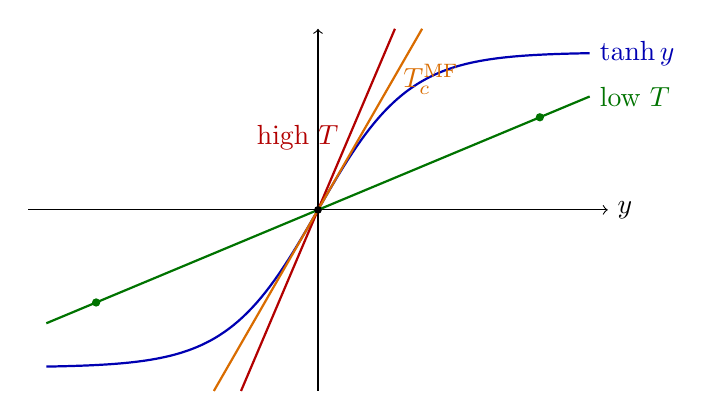
\begin{tikzpicture}[x=1.15cm,y=2.0cm]
\draw[->] (-3.2,0) -- (3.2,0) node[right] {$y$};
\draw[->] (0,-1.15) -- (0,1.15);
\draw[thick,blue!70!black,domain=-3:3,samples=120]
  plot (\x,{tanh(\x)}) node[right] {$\tanh y$};
\draw[thick,red!70!black] (-0.85,-1.15) -- (0.85,1.15)
  node[pos=0.70,left] {high \(T\)};
\draw[thick,orange!85!black] (-1.15,-1.15) -- (1.15,1.15)
  node[pos=0.86,right] {\(T_c^{\rm MF}\)};
\draw[thick,green!45!black] (-3,-0.72) -- (3,0.72)
  node[right] {low \(T\)};
\fill (0,0) circle (1.4pt);
\fill[green!45!black] (-2.45,-0.588) circle (1.5pt);
\fill[green!45!black] (2.45,0.588) circle (1.5pt);
\end{tikzpicture}
\caption{자기일관성을 그래프로 설명하는 논증을 정규화해 다시 그린 그림.}
\end{figure}

영이 아닌 가지는 연속적으로 나타난다. 상전이 부근에서는
\begin{equation}
\tanh(Km)=Km-\frac{(Km)^3}{3}+O(m^5).
\end{equation}
\(K>1\)일 때, 작은 영이 아닌 해는 다음을 만족한다.
\begin{equation}
m^2\simeq \frac{3(K-1)}{K^3}.
\end{equation}
따라서 평균장 이론은 익숙한 제곱근형 발현을 예측한다. \(m\propto(T_c-T)^{1/2}\)

그래프를 어떻게 그렸는지에 의존하지 않고도 안정성에 관한 진술을 할 수 있다. \(m\)에 무관한 상수를 제외하면, 스핀당 평균장 자유에너지는 다음과 같다.
\begin{equation}
f_{\rm MF}(m)
=dJm^2-\frac{1}{\beta}
\log\!\left[2\cosh(2\beta dJm)\right].
\label{eq:mf-free-energy}
\end{equation}
그 정지 조건은
\begin{equation}
\frac{\partial f_{\rm MF}}{\partial m}
=2dJ\left[m-\tanh(2\beta dJm)\right]=0.
\end{equation}
이다. \(T_c^{\rm MF}\)보다 높은 온도에서는 \(m=0\)가 최소점이다. 그보다 낮은 온도에서는 원점이 국소 최대점이고, 0이 아닌 두 해가 축퇴된 최소점이다. 교점의 기하와 자유에너지의 열역학은 같은 결론을 말해 준다.

\begin{classroomqa}
\audiencequestion{해 \(m=0\)는 \(T_c^{\rm MF}\) 아래에서도 교점으로 남아 있습니다. 왜 0이 아닌 가지가 물리적인 해인가요?}
\lecturerresponse{절대영도에서 온도를 높여 가는 계는 이미 자화된 가지에 놓인다. 더 엄밀히 말하면, 상전이 아래에서 평균장 자유에너지는 \(\pm m_0\)에서 최소점을 가지며 \(m=0\)는 최대점이 된다. 그러면 무한소의 외부장이 최소점 하나를 선택해 겉으로 보이는 모호성을 없앤다. \lecturetimestamp{01:11:34--01:12:18}}
\end{classroomqa}

\section{평균장이 1차원에서 실패하는 이유}

\(d=1\)을 식~\eqref{eq:mean-field-tc}에 대입하면 \(T=2J\)에서 상전이가 일어난다고 예측하여, 정확한 1차원 해와 모순된다. 대수적으로 발산하는 항은 없다. 이 근사는 이웃 둘이 큰 통계적 열저장고가 아니며, 1차원의 영역벽이 특별한 엔트로피를 갖기 때문에 실패한다.

모든 스핀이 위쪽을 향하는 상태에서 시작하자. 결합 하나가 끊어지면 에너지가 \(-J\)에서 \(+J\)로 바뀌므로, 끊어진 결합 하나의 에너지 비용은
\begin{equation}
\Delta E_{\rm bond}=2J.
\end{equation}
이다. 정사각 격자에서 스핀 하나를 뒤집으면 결합 네 개가 끊어지고 비용은 \(8J\)이다. 뒤집힌 스핀 두 개가 서로 이웃하면 둘레에 끊어진 결합이 여섯 개 생겨 비용은 \(12J\)이다. 반면 서로 멀리 떨어진 두 스핀을 뒤집으면 결합 여덟 개가 끊어져 비용은 \(16J\)이다.

\begin{figure}[ht]
\centering
\includegraphics[width=0.82\textwidth]{lecture_09_figure_09.png}
\caption{정사각 격자에서 이웃한 두 스핀의 방향을 뒤집은 모습. 두 스핀이 공유하는 결합은 만족되므로 경계에는 끊어진 결합이 여섯 개 남는다.}
\lectureframe{01:17:30}
\end{figure}

따라서 2차원에서 조밀하게 모인 반전 영역은 경계 길이에 비례하는 에너지 비용을 치른다.
\begin{equation}
\Delta E_{\rm 2d}=2J\,|\partial D|.
\end{equation}
영역이 커지면 일반적으로 경계도 길어진다.

1차원에서는 다르다. 길이가 얼마든 연결된 반전 구간에는 영역벽이 두 개뿐이다.
\begin{equation}
\Delta E_{\rm 1d}=2(2J)=4J.
\label{eq:one-d-domain-cost}
\end{equation}

\begin{figure}[ht]
\centering
\includegraphics[width=0.82\textwidth]{lecture_09_figure_10.png}
\caption{영역벽 두 개만 경계로 갖는 1차원의 긴 반전 구간.}
\lectureframe{01:19:10}
\end{figure}

\(N\)개의 격자점으로 된 사슬에서는 이런 구간의 두 영역벽을 선택하는 방법이 대략 \(N^2\)가지다. 두 영역벽 사이의 거리가 멀어져도 에너지는 증가하지 않는다. 온도가 양수이기만 하면 엔트로피 때문에 임의로 큰 반전 영역이 생긴다. 2차원에서는 충분히 낮은 온도에서 경계 에너지가 윤곽의 엔트로피를 이길 수 있다. 이 에너지와 엔트로피의 경쟁은 평균장이 \(d=1\)과 \(d=2\)를 같은 계수의 서로 다른 수치로만 다룰 때 포착하지 못하는 기하학적 사실이다.

\begin{classroomqa}
\audiencequestion{반전된 스핀들이 서로 이웃해야만 영역벽 두 개의 일정한 에너지 비용이 드나요?}
\lecturerresponse{그렇다. 여기서 말하는 것은 하나로 연결된 반전 구간이다. 뒤집힌 스핀들이 여러 구간으로 나뉘면 구간 하나마다 영역벽 두 개가 더 생긴다. 중요한 점은 구간 하나가 임의로 길어져도 영역벽은 두 개뿐이라는 것이다. \lecturetimestamp{01:18:32--01:18:40}}
\end{classroomqa}

\begin{classroomqa}
\audiencequestion{평균장 방정식 자체로는 \(d=1\)과 \(d=2\) 사이에 질적인 차이가 없어 보입니다. 그것이 문제인가요?}
\lecturerresponse{그렇다. 평균장 이론은 양의 \(d\)마다 상전이를 예측하므로 1차원에서는 질적으로 틀린 답을 준다. 평균장 유도는 요동이 약한 이웃이 많다고 가정하며 영역벽의 기하를 버렸다. 1차원 문제를 결정하는 것은 정확한 결합 변수 해이지, 평균장 치환 \(d=1\)가 아니다. \lecturetimestamp{01:19:44--01:20:28}}
\end{classroomqa}

\section{외부장이 상을 선택한다}

\(h>0\)일 때 \(\sigma=+1\)를 선호하는 규약으로 균일한 외부장 \(h\)을 추가하자.
\begin{equation}
H=-J\sum_{\langle ij\rangle}\sigma_i\sigma_j
-h\sum_i\sigma_i.
\label{eq:ising-with-field}
\end{equation}
선택한 스핀 하나의 평균장 에너지는
\begin{equation}
E_i^{\rm MF}=-(2dJm+h)\sigma_i,
\end{equation}
이고 자기일관 방정식은 다음과 같이 된다.
\begin{equation}
\boxed{m=\tanh\!\left[\beta(2dJm+h)\right]}.
\label{eq:self-consistency-field}
\end{equation}
\(K=2\beta dJ\)와 \(y=Km\)를 사용하면
\begin{equation}
\frac{y}{K}=\tanh(y+\beta h).
\label{eq:shifted-graph}
\end{equation}

\begin{figure}[ht]
\centering
\includegraphics[width=0.82\textwidth]{lecture_09_figure_11.png}
\caption{자기일관 방정식에 외부장 항을 추가하고 그래프를 평행 이동해 나타낸 그림.}
\lectureframe{01:26:20}
\end{figure}

\begin{classroomqa}
\audiencequestion{외부장은 왜 쌍곡탄젠트 안에만 더하나요? 좌변도 바꿔야 하지 않나요?}
\lecturerresponse{좌변은 가정한 자화 \(m\), 즉 \(y/K\)이다. 우변은 전체 유효장 \(2dJm+h\) 속에 놓인 스핀의 자화로 계산한 값이다. 자기일관성은 이 두 양을 같게 놓는다. \(y=Km\)를 고정된 정의로 유지하면 새 항은 \(\tanh(y+\beta h)\)의 인수에만 들어간다. \lecturetimestamp{01:23:46--01:26:18}}
\end{classroomqa}

\begin{classroomqa}
\audiencequestion{같은 그래프 변화를 \(\tanh\) 곡선을 이동하는 대신 직선들을 움직이는 방식으로 설명할 수 있나요?}
\lecturerresponse{그렇다. \(\tanh y\)를 고정한 채 방정식을 다시 써서 직선의 절편이 0이 아니도록 할 수 있다. 교점은 똑같다. 두 설명의 차이는 방정식의 어느 쪽을 고정된 그래프로 택하느냐뿐이다. \lecturetimestamp{01:35:07--01:36:26}}
\end{classroomqa}

\(h\neq0\)이면 원점은 더 이상 해가 아니다. \(T_c^{\rm MF}\)보다 낮은 온도에서는 아무리 작은 양의 장도 양의 가지를 선택하고, 음의 장은 음의 가지를 선택한다.

\begin{figure}[ht]
\centering
\includegraphics[width=0.82\textwidth]{lecture_09_figure_12.png}
\caption{약한 외부장은 대칭인 교점을 없애고 자화된 가지 하나를 선택한다.}
\lectureframe{01:36:22}
\end{figure}

올바른 서술을 위해서는 극한을 취하는 순서가 중요하다. 유한한 계에서 \(h=0\)이면 스핀 반전 대칭이 있으므로 전체 평형 앙상블에서 \(\expect{m}=0\)이다. 자발 자화는 다음과 같다.
\begin{equation}
m_{\rm sp}
=\lim_{h\to0^+}\lim_{N\to\infty}\expect{m}_{N,h},
\end{equation}
여기서는 열역학적 극한을 먼저 취한다. 무한소 외부장의 부호를 반대로 하면 \(-m_{\rm sp}\)를 얻는다. 전체 장 에너지의 차이는 \(Nh\)에 비례하므로, 아무리 작은 장도 거시적인 시료에서는 결정적인 영향을 준다.

해당하는 자유에너지를 보면 기울어진 모양이 드러난다.
\begin{equation}
f_{\rm MF}(m;h)
=dJm^2-\frac{1}{\beta}
\log\!\left[2\cosh\!\left(\beta(2dJm+h)\right)\right].
\end{equation}
\(h=0\)에서는 두 우물이 같은 깊이다. 양의 \(h\)는 양의 \(m\) 우물을 낮추고 음의 \(m\) 우물을 높인다. 스핀당 섭동은 아주 작아도 \(N\)을 곱한 전체 선호는 거시적일 수 있다.

\begin{classroomqa}
\audiencequestion{외부장이 계속 가해지고 있다면 자화는 정말 자발적인 것인가요?}
\lecturerresponse{장은 어느 한 분지를 선택하는 데만 쓰입니다. \(T<T_c\)에서 계의 크기를 무한대로 보낸 다음 \(h\to0^+\)이 되도록 합니다. 선택장이 사라지더라도 자화는 유한한 값으로 남습니다. 극한을 취하는 부호를 반대로 하면 반대쪽 상이 선택됩니다. \lecturetimestamp{01:33:15--01:34:18}}
\end{classroomqa}

\begin{classroomqa}
\audiencequestion{전이 아래에서 평균이 0인 해는 실제로 불가능한가요, 아니면 불안정할 뿐인가요?}
\lecturerresponse{장이 정확히 0일 때 두 방향에 같은 가중치를 주는 대칭적인 유한 부피 앙상블은 가능하며, 평균은 0입니다. 안정하지 않은 것은 이 앙상블이 하나의 거시적 상으로 존재하는 경우입니다. 아무리 작은 장이라도 계의 크기에 비례하는 에너지 균형을 바꾸어 한 방향을 선택합니다. 열역학적 극한을 취한 뒤에는 장을 제거해도 선택된 자화가 남습니다. \lecturetimestamp{01:34:25--01:35:06}}
\end{classroomqa}

\begin{classroomqa}
\audiencequestion{무한 온도에서 외부장에 편향된 해는 어떻게 되는가?}
\lecturerresponse{유한한 \(h\)를 고정하면, \(K=2\beta dJ\)와 \(\beta h\)는 모두 \(T\to\infty\)일 때 사라진다. 그러면 ~\eqref{eq:self-consistency-field}은 \(m\to0\)를 준다. 약한 외부장은 저온 가지를 선택하지만, 무한한 열적 요동에 맞서 질서를 유지할 수는 없다. \lecturetimestamp{01:27:39--01:29:51}}
\end{classroomqa}

\begin{classroomqa}
\audiencequestion{온도와 그래프의 이동량을 함께 바꿀 때, 교점이 어디로 이동하는지 어떻게 확신할 수 있나요?}
\lecturerresponse{교점이 움직이는 그림보다 음함수 방정식이 더 확실한 지침입니다. 저온에서 양의 \(h\)를 가하면 안정한 해는 \(m=+1\)에 가까워집니다. 고온에서는 탄젠트를 전개하면
\[
m\simeq \beta(2dJm+h)
\quad\Longrightarrow\quad
m\simeq \frac{\beta h}{1-2\beta dJ},
\]
\(\beta\to0\)일 때 0으로 갑니다. 따라서 안정한 분지는 전이 아래에서 불안정한 원점에 머무르지 않고, 저온의 정렬된 극한과 고온의 약한 편극 상태를 이어 줍니다. \lecturetimestamp{01:29:53--01:33:04}}
\end{classroomqa}

\section{자기 역전은 다른 문제다}

\begin{classroomqa}
\audiencequestion{지구 자기장은 무엇 때문에 방향이 바뀌나요?}
\lecturerresponse{이 질문은 평형 이징 모형의 범위를 벗어납니다. 지구의 주된 자기장은 지구 다이너모에 의해 생성됩니다. 외핵에서 전기 전도성 유체의 대류와 회전이 전류와 자기장을 유지합니다. 자기장 역전은 비선형 다이너모가 불규칙하게 재편되는 현상이지, 고체 철에서 강자성 영역이 단순히 뒤집히는 현상이 아닙니다. 역전이 일어나는 구체적인 시점은 하나의 평형 질서 매개변수로 설명할 수 없으므로, 여기서 솔직한 답은 이징 계산으로 그 촉발 요인을 설명할 수 없다는 것입니다. 유용한 연결점은 서로 반대인 두 거시적 방향을 가진 계에서 그 두 상태 사이에 불안정성이 생길 수 있다는 일반적인 사실뿐입니다.\footnote{\href{https://science.nasa.gov/science-research/earth-science/earths-magnetosphere-protecting-our-planet-from-harmful-space-energy/}{지구 다이너모에 관한 NASA 개요}와 \href{https://www.usgs.gov/programs/geomagnetism/introduction-geomagnetism}{미국 지질조사국의 지자기에 관한 입문 자료}를 참조하세요.} \lecturetimestamp{01:38:39--01:40:32}}
\end{classroomqa}

정확한 사슬 모형과 평균장 격자 모형은 이제 뚜렷하게 다른 두 답을 준다. 한 차원에서는
\begin{equation}
\expect{\sigma_i\sigma_{i+r}}
=\left[\tanh(\beta J)\right]^r
\longrightarrow0
\qquad (T>0),
\end{equation}
유한한 에너지를 가진 영역벽이 임의로 긴 반전 구간을 서로 분리할 수 있기 때문이다. 반면 이웃이 많으면 자기일관적 장은 다음 값보다 낮은 온도에서 안정한 영이 아닌 해를 허용한다.
\begin{equation}
T_c^{\rm MF}=2dJ.
\end{equation}
이 차이는 단순히 대수적인 데 그치지 않는다. 기하학적 구조, 에너지, 엔트로피, 중복성이 서로 경쟁한 결과다. 즉, 오류가 제약 없이 퍼질 수 있는지, 아니면 주변 격자가 이를 바로잡을 수 있는지의 차이다.